\documentclass[11pt]{article}
\usepackage[margin=1.1in]{geometry}
\usepackage{amsmath,amssymb,amsthm}
\usepackage{booktabs}
\usepackage{array}
\usepackage{tabularx}
\usepackage[protrusion=true,expansion=false]{microtype}
\usepackage[table]{xcolor}
\usepackage{enumitem}
\usepackage{titlesec}
\usepackage{tikz}
\usepackage{float}
\usetikzlibrary{arrows.meta,positioning,calc}
\usepackage{hyperref}

\hypersetup{colorlinks=true, linkcolor=blue!60!black, urlcolor=blue!60!black, citecolor=blue!60!black}
\usepackage[skip=0.6\baselineskip, indent=0pt]{parskip}

\titleformat{\section}{\large\bfseries}{\thesection.}{0.7em}{}
\titleformat{\subsection}{\normalsize\bfseries}{\thesubsection.}{0.6em}{}
\titleformat{\part}[display]{\centering\Large\bfseries}{Part \thepart}{0.3em}{}

\newcommand{\vmax}{V_{\max}}
\newcommand{\Tc}{T_{\mathrm{close}}}
\newcommand{\tx}[1]{\texttt{#1}}
\newcolumntype{L}{>{\raggedright\arraybackslash}X}

\renewcommand{\arraystretch}{1.3}
% float pages: floats from the top, not spread over the page
\makeatletter
\setlength{\@fptop}{0pt}
\setlength{\@fpsep}{1.5\baselineskip}
\setlength{\@fpbot}{0pt plus 1fil}
\makeatother
\rowcolors{1}{}{black!5}

\definecolor{coop}{RGB}{232,245,233}
\definecolor{chainc}{RGB}{255,228,225}
\definecolor{hubc}{RGB}{255,243,214}

\title{\textbf{Lichen as built}\\the BABE gadget, the hub's ledger and the exit\\[2pt]\large draft}
\author{waxwing}
\date{Version 0.1, October 2026\\[2pt]\small a companion to \emph{Lichen}, version 0.4~\cite{lichen}}

\begin{document}
\maketitle

\begin{abstract}
This companion to Lichen~\cite{lichen} gathers what is built and
measured, in two parts. Part~I is the verification gadget, BABE~\cite{babe},
which serves any L2. BABE's statement is fixed when the parties set up,
while Alice chooses the amount $b$ only when she withdraws; so the amount
moves into the witness, together with the hub's one-time signature on
it, which the hub must give on chain for exactly the amount Alice
asserted there, or lose. BABE's cryptography is unchanged. We give the
transaction graph as built, a tower that holds none of Alice's keys, the
setup by verifiable secret sharing (19~seconds per contract on one
laptop; the user keeps about 240~MiB), and the measurements: on Mutinynet
with a real RISC Zero proof, a true claim challenged by the hub and
answered took 30.5~kvB in five transactions, against BitVMX's
100--212~kvB in 23--25; unchallenged, 9.7~kvB in four; a false claim,
29.9~kvB in five. Part~II is lichen's own L2, in which the hub is also
the sequencer, so that the withdrawal statement must enforce what a
separate L2 would vouch for: validity, by a chain of proofs; one history,
final on Bitcoin, by a chain of single-use seals with the contract's
work on top; and an exit from a state already anchored, against an
operator that censors its users or vanishes, which the hub may answer
only with a counter. An exit's dispute is about 15~kvB. The worst case
falls on Alice: proving a forged counter false verifies a Groth16 proof
inside RISC Zero, 56.3M cycles, about an hour on a laptop, and we set out
the alternatives. The security argument is still a sketch, and data
availability is the main open problem.
\end{abstract}

\tableofcontents

\section{Scope}
\label{sec:scope}

The main paper~\cite{lichen} describes a contract between a user, Alice,
and a hub: a 2-of-2 output holding her deposit, the hub's liquidity up to
a cap $\vmax$, and two reserves. The hub's tokens on an L2 are
collateralised by it; a withdrawal of $b$ is a return of $b$ tokens to
the hub tied to the contract $c$, folded cooperatively or, if the hub
refuses or is offline, enforced on Bitcoin by a verification gadget. The
withdrawal statement is a predicate the L2 supplies,
$\mathcal{R}_L(\mathcal{D}, c, \ldots; w)$, with $\mathcal{D}$ the
deployment's parameters and $w$ the witness; how the L2 makes its
account of its ledger trustworthy is its own business. This companion
gathers what lichen builds~\cite{lichencode} on either side of that
interface:
\begin{itemize}[leftmargin=1.5em]
\item \emph{Part~I, the gadget}: BABE, with the amount authenticated by
  the hub, as built and measured. It serves any $\mathcal{R}_L$.
\item \emph{Part~II, lichen's own L2}: a ledger whose sequencer is the
  hub, and the statement that must then enforce validity, finality and
  an exit against it.
\end{itemize}
lichen's first gadget was BitVMX's interactive search~\cite{bitvmx},
described and measured in its own companion~\cite{lichenbitvmx}, which
is no longer maintained; it is the comparison throughout Part~I.

What is ours is narrow in Part~I: the binding of a late-chosen amount by
the hub's authentication (Section~\ref{sec:auth}), first put forward in a
discussion on Delving Bitcoin~\cite{delving}; the transaction graph and
the setup by verifiable secret sharing, as built; and the measurements.
BABE, its witness encryption and its garbled circuit are its
authors'~\cite{babe,gkpw24,argo}; the problem of public inputs that are
known only at proving time has been treated at the cryptographic layer by
GOAT's researchers~\cite{goat}. Part~II is lichen's design throughout.

Figures marked (BABE) are the BABE paper's measurements, taken from its
revised version (October 2026); figures marked (lichen) are measured in
lichen's proof of concept, on regtest under mainnet's relay policy or on
Mutinynet as stated; the rest are estimates, marked (est.). Where the
design's estimates, made before the gadget was built, differ from the
measurements, they are kept beside them. Proving times are on one
14-core Apple M4 Pro laptop, on its CPU (the RISC Zero version we use
has no Metal prover), or on a rented 4-vCPU x86 server, as stated.

\part{The gadget}

\section{BABE in brief}
\label{sec:babe}

Groth16's verification, written additively in the target group, is
\[
  e(\pi_1, \pi_2) + e(\pi_3, \delta) = T, \qquad
  T = e(\alpha, \beta) + e(L, \gamma), \qquad
  L = \mathit{IC}_0 + \textstyle\sum_i s_i\, \mathit{IC}_i,
\]
where $\pi_1, \pi_2, \pi_3$ are the proof, $s_i$ the public inputs, and
the rest the verifying key. Witness encryption (WE) lets a party encrypt
a message so that only a holder of a valid proof can decrypt it. For
pairing relations \emph{linear} in the witness there is a simple
scheme~\cite{gkpw24}: for a secret scalar $r$, publish $r$ times the
public elements; a holder of the witness pairs it against them and
obtains $r\,T$, which unmasks the message. Groth16's check is not linear
in the witness, because of $e(\pi_1, \pi_2)$. BABE's idea is to supply
$r\pi_1$ by two-party computation once $\pi_1$ is known:
\begin{itemize}[leftmargin=1.5em]
\item \emph{Setup.} The verifier picks $r$ and a message $\mathit{msg}$,
  publishes the WE ciphertext ($r\delta$ and $\mathit{msg}$ masked by
  $r\,T$; 480~bytes), commits to $\mathit{msg}$ by its hash, and
  garbles a circuit computing $r\pi_1$ from the bits of $\pi_1$, with $r$
  inside. The circuit is small because group addition to a fixed point
  is linear in a six-term feature vector of the point, so all but a
  point-validation gadget is a decomposable randomized encoding with no
  garbled tables, after Argo MAC~\cite{argo}: 22~MiB per instance, 175~ms
  to make (BABE).
\item \emph{Assert.} The prover posts $\pi_1$ under a Lamport signature
  (508 bits).
\item \emph{ChallengeAssert.} To contest, the verifier must post the
  circuit's input labels for exactly those bits; a script checks that
  its labels and the prover's Lamport signature sign the same value. (A
  garbled circuit's input labels \emph{are} a Lamport signature of its
  input.)
\item The prover evaluates the circuit, obtains $r\pi_1$, completes the
  decryption with $\pi_2$ and $\pi_3$, and, if the proof is valid,
  publishes $\mathit{msg}$ (\emph{WronglyChallenged}), which blocks the
  verifier's \emph{Failure}; after a timelock $\Delta_2$ the prover's
  \emph{Success} pays. If the verifier never challenges, Success pays
  after $\Delta_2$ anyway. Failure needs $\Delta_1$ after the challenge.
\end{itemize}
On chain, a contested valid proof costs Assert 9,240~vB, ChallengeAssert
17,400~vB and WronglyChallenged 149~vB (BABE), with one set of labels.
Against a verifier who might garble wrongly (one whose circuit never lets
the prover decrypt), the prover checks the garbling by cut-and-choose:
for example 2,268 instances of which 4 are kept, 1~min~37~s and 1.8~GB at
peak on a 16-thread laptop (BABE). Without more, the verifier must then
post 4 sets of labels; \emph{soldering}, a SNARK proving the kept
instances' labels consistent, brings it back to one at about 12~minutes
more of setup (BABE); verifiable secret sharing does the same in seconds,
and is what lichen builds (Section~\ref{sec:vsss}). The WE is
extractable, proved in the generic group model. The protocol is proved
robust (an honest prover is paid) and knowledge-sound (a prover who is
paid knows a witness) for a setup that both parties run honestly.
Against a verifier who garbles wrongly, cut-and-choose is argued,
failing with probability at most $2^{-40}$ for the parameters above, but
not proved (BABE).

\section{Where BABE fits in lichen}
\label{sec:fit}

\paragraph{The proving stack is unchanged.} lichen's withdrawal proof is
a Groth16 proof over BN254: RISC Zero's recursion compresses the guest's
STARK receipts into a succinct receipt, and RISC Zero's shrink-wrap
proves that receipt's verification in Groth16, with RISC Zero's single
trusted setup~\cite{risc0}. BABE verifies exactly such a proof. Any proofs
the L2's statement composes, such as lichen's chain proofs, and the wrap
stay as they are; BABE's withdrawal guest is the withdrawal statement
with one more check and a different journal (Section~\ref{sec:auth}).

\paragraph{The roles.} Alice, who claims her withdrawal, is BABE's
prover; the hub, the only party a false claim can rob, is its verifier,
and so the garbler. BABE is a protocol between one prover and one
verifier, both known at setup, which is what a lichen contract is: no
committee, no open set of challengers, and no one else's funds in the
output. Designs whose challengers are not known in advance pay heavily
to approximate this; a bilateral contract has it for free.

\paragraph{Setup is per contract, and two-party.} The hub garbles for
each contract; Alice checks the garbling by cut-and-choose and keeps the
finalized instances. This replaces nothing in lichen's trust model: as
under BitVMX, the contract is set up by its two parties alone. What it
adds is cost at opening (Section~\ref{sec:setup}).

The two parties' conduct at setup protects different funds. A hub that
garbles wrongly could refuse a valid withdrawal, since Alice could never
decrypt; cut-and-choose is what rules this out, so Alice's funds rest on
it. Alice's part in setup is small (her keys, her pre-signatures, and
which instances to keep), and every secret is the hub's, so the hub's
funds rest on the proving phase, where BABE's proofs apply.

\paragraph{One-shot.} Revealing labels spends a garbled circuit's
security, so a BABE instance settles one claim. A lichen contract has at
most one withdrawal, after which it closes; renewal is a new contract
with a new setup.

\section{The fixed statement}
\label{sec:fixed}

BABE's ciphertext is built from $T$, and $T$ contains $e(L, \gamma)$,
the combination of the public inputs. So the whole public input is fixed
at setup. For a RISC Zero proof that input is the claim digest, a hash
over the image id and the journal; under BitVMX the journal is
$b \,\|\, c \,\|\, \mathcal{D}$, so setup would fix $b$, which Alice chooses only
when she withdraws. The ways round it that we know of:
\begin{itemize}[leftmargin=1.5em]
\item \emph{Supply $rL$ at proving time} for the asserted public input
  only, by envelopes opened with labels the verifier reveals per bit.
  With a single scalar public input this fails: the points
  $r\,2^j\mathit{IC}$ share one base, so one of them gives away
  $r\,\mathit{IC}$ and with it the ciphertext for any input. It needs
  each bit to be its own public input with an independent base, so a
  custom Groth16 wrap and its own trusted setup, and a garbled SHA-256
  between $b$ and RISC Zero's digest.
\item \emph{Deferred binding at the cryptographic layer}, as GOAT's
  researchers propose~\cite{goat}: a blinding point and further garbled
  circuits for the dynamic part of the input, one of them about 200
  million gates, and a larger challenge transaction.
\item \emph{One instance per digit value}: decompose $b$ in base $B$ and
  set up a fixed statement for each nonzero digit at each position. A
  dispute then proves each nonzero digit separately; base 16 for a
  14-bit amount means 60 setups per contract and up to four disputes.
\item \emph{Refresh the statement} whenever Alice's balance changes,
  which needs contracts in channels so that the refresh is off chain,
  and a setup per change of balance.
\item \emph{Set up only when withdrawing.} Rejected: a hub that declined
  the setup would leave Alice's tokens without collateral, which breaks
  the contract's first property, that within its cap Alice trusts the
  hub for nothing.
\end{itemize}
We take none of these. Section~\ref{sec:auth} moves $b$ into the
witness instead, so one fixed statement, set up once per contract,
serves any amount, and Script reads $b$ from the parties' signatures.

\section{Authenticated amounts}
\label{sec:auth}

\subsection{The statement}

Let the hub hold, per contract, a one-time signing key $pk_H$, fixed at
setup. The statement proved becomes
\[
  \exists\, b, w, \sigma_H:\quad
  \mathrm{Verify}(pk_H, b, \sigma_H) = 1 \;\wedge\;
  \mathcal{R}_L(\mathcal{D}, c; b, w) = 1,
\]
where $\mathcal{R}_L$ is the L2's withdrawal statement unchanged (a
return of $b$ to the hub tied to the contract $c$; for lichen's own L2,
the statement of Part~II) and $w$ its witness. The journal holds only
values fixed when the contract opens: $c \,\|\, \mathcal{D} \,\|\, H(pk_H)$.
The claim digest, and so BABE's statement, is then fixed at setup, while
$b$ is free until Alice withdraws.

\subsection{The flow}

\begin{enumerate}[leftmargin=1.5em]
\item \emph{Request.} Alice asserts $b$ on chain under her one-time key
  for it, as under BitVMX.
\item \emph{Response.} The hub must sign the same $b$ under $pk_H$, on
  chain, within its window $w_H$. The response's script verifies both
  signatures and checks, digit by digit, that they sign the same value.
  If the hub is silent, Alice's timeout pays her the asserted $b$, as
  the hub's silence does under BitVMX.
\item \emph{Proof.} Alice proves the statement, using the hub's
  signature as part of her witness, and wraps the proof. Her wallet
  stops after the response with the hub's signature written out for the
  prover, and resumes when given the proof; she has until an absolute
  deadline $T_A$, shortly before $\Tc$ (Section~\ref{sec:graph}).
\item \emph{BABE.} Assert, ChallengeAssert, WronglyChallenged or
  Failure, as in Section~\ref{sec:babe}.
\item \emph{Payout.} Success pays through the bit outputs, which read
  $b$ from Alice's signature, as under BitVMX.
\end{enumerate}

\subsection{Why the amount is bound}
\label{sec:binding}

The hub's signature is not a judgement. It means ``this is the amount
being adjudicated'', not ``this withdrawal is valid'', and an honest hub
gives it mechanically for whatever Alice asserted, true or false. Three
links bind the amount proved to the amount paid:
\begin{itemize}[leftmargin=1.5em]
\item the proof's $b$ is the hub's, because the guest checks the hub's
  signature;
\item the hub's $b$ is Alice's on-chain $b$, because the response's
  script compares them digit by digit;
\item Alice's $b$ is the one paid, because the bit outputs read her
  signature, and a second signature from her under the same key forfeits
  them (\tx{equiv\_b}).
\end{itemize}
Suppose Alice asserts 100 but can prove a withdrawal of only 10. She has
the hub's signature on 100 and no valid withdrawal of 100, or a valid
withdrawal of 10 and no signature on 10. Neither satisfies the
statement.

\paragraph{The authenticator must be the hub.} Alice's own signature on
$b$ inside the witness would bind nothing: she could sign 10 privately
for the proof and 100 on chain for the payout, and the private
signature, hidden in a zero-knowledge witness, would never be seen, so
the equivocation could not be shown. A key she does not hold, used only
on chain, is what carries the on-chain value into a fixed statement. The
hub must therefore never sign a second value under $pk_H$, not even off
chain; its key is used once, in the response, and the cooperative fold
never touches it.

\paragraph{The payout could check both signatures.} Since the hub's
signature on $b$ is on chain, each bit output could require both
parties' signatures on the same value: Alice's leaf with bit $i$ set, the
hub's with it clear. Neither can then spend with a value the other did
not sign, which removes \tx{equiv\_b} and Alice's wait $\delta$ at about
the same script cost. This is not built: the bit outputs are BitVMX's.

\subsection{The guest}

The guest takes $b$ and $\sigma_H$ as private inputs, checks $\sigma_H$
against $pk_H$, runs the withdrawal statement, and commits $c$,
$\mathcal{D}$ and $pk_H$'s digest. LN-GAP's one-time signatures chain
\texttt{HASH160}, RIPEMD-160 of SHA-256, which has no accelerator in RISC
Zero's zkVM; the hub's key instead chains SHA-256, which the zkVM
accelerates and Script checks with \texttt{OP\_SHA256}, at 32 bytes a
chain value. Alice's key for $b$ stays LN-GAP's, so the response's
script verifies one signature of each kind. With lichen's statement
(Section~\ref{sec:withdrawal}) the guest runs in 482k user cycles
against the plain withdrawal guest's 333k, one segment either way
(lichen); the design estimated the check at a few thousand cycles.

\subsection{Security, as a sketch}
\label{sec:security}

The statement cannot say that the hub signed $b$, only that a valid hub
signature on $b$ exists, and one exists for every $b$; only the hub can
compute it. So what binds the amount is not that a false statement
cannot be proved but that the prover must \emph{know} a witness: that
whoever is paid knows one, which then contains a hub signature, which
unforgeability then forces to be on the asserted amount. The pipeline
already relies on this: lichen's chain proof's checks of users'
signatures bind in the same way.

BABE gives the first step. Its knowledge soundness (Definition 9 of
\cite{babe}) states that for any NP relation, a prover who gets the
Success transaction onto the chain knows a witness, in the sense that an
extractor recovers one from its view; it is proved for an honestly run
setup (its Definition 16 and Theorem 8). Here the relation is the
statement above, through two more layers: Groth16 is knowledge-sound
(in the generic or algebraic group model), so the Groth16 proof yields
a valid RISC Zero receipt; RISC Zero's STARKs are arguments of knowledge
(in the random-oracle model), so the receipt yields the guest's input,
$(b, w, \sigma_H)$. If $b \ne b^*$, the asserted amount, then $\sigma_H$
is a signature under $pk_H$ on a message the hub never signed, and the
hub signed exactly one: a forgery against a one-time signature.

What remains to be written properly:
\begin{itemize}[leftmargin=1.5em]
\item BABE proves knowledge soundness for an honestly run setup, not yet
  for one in which the prover takes part. Alice's part is small and
  every secret is the hub's (Section~\ref{sec:fit}), so we expect the
  extension to be routine.
\item The hub's signature arrives during the proving phase, after the
  statement is fixed, and depends on Alice's own assertion: the
  extraction must hold with the signature in the prover's view, which
  BABE's definition allows but which should be checked against its
  proof.
\item The composition of extractors across BABE, Groth16 and the STARKs,
  under BABE's restriction to benign auxiliary input.
\end{itemize}

\section{The transaction graph}
\label{sec:graph}

\begin{figure}[!htp]
\centering
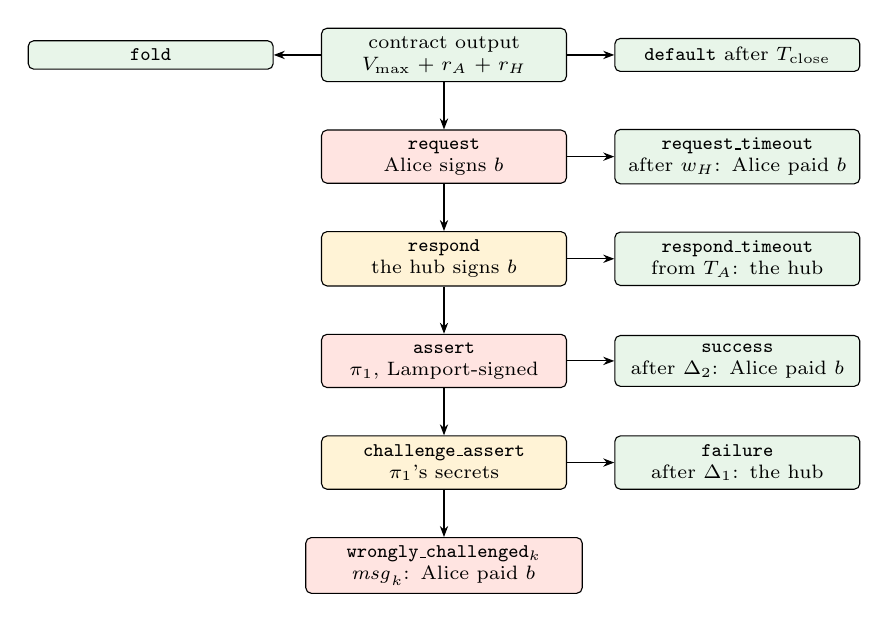
\begin{tikzpicture}[
  font=\scriptsize,
  tx/.style={draw, rounded corners=2pt, align=center, inner sep=3pt, text width=#1},
  tx/.default=29mm,
  >={Stealth[length=4pt]},
  node distance=6mm and 6mm,
]
\node[tx, fill=coop] (c) {contract output\\$\vmax + r_A + r_H$};
\node[tx, fill=coop, left=of c] (fold) {\tx{fold}};
\node[tx, fill=coop, right=of c] (def) {\tx{default} after $\Tc$};
\node[tx, fill=chainc, below=of c] (req) {\tx{request}\\Alice signs $b$};
\node[tx, fill=coop, right=of req] (rt) {\tx{request\_timeout}\\after $w_H$: Alice paid $b$};
\node[tx, fill=hubc, below=of req] (resp) {\tx{respond}\\the hub signs $b$};
\node[tx, fill=coop, right=of resp] (rspt) {\tx{respond\_timeout}\\from $T_A$: the hub};
\node[tx, fill=chainc, below=of resp] (as) {\tx{assert}\\$\pi_1$, Lamport-signed};
\node[tx, fill=coop, right=of as] (succ) {\tx{success}\\after $\Delta_2$: Alice paid $b$};
\node[tx, fill=hubc, below=of as] (ca) {\tx{challenge\_assert}\\$\pi_1$'s secrets};
\node[tx, fill=coop, right=of ca] (fail) {\tx{failure}\\after $\Delta_1$: the hub};
\node[tx=33mm, fill=chainc, below=of ca] (wc) {\tx{wrongly\_challenged}$_k$\\$\mathit{msg}_k$: Alice paid $b$};
\draw[->] (c) -- (fold);
\draw[->] (c) -- (def);
\draw[->] (c) -- (req);
\draw[->] (req) -- (rt);
\draw[->] (req) -- (resp);
\draw[->] (resp) -- (rspt);
\draw[->] (resp) -- (as);
\draw[->] (as) -- (succ);
\draw[->] (as) -- (ca);
\draw[->] (ca) -- (fail);
\draw[->] (ca) -- (wc);
\end{tikzpicture}
\caption{The dispute's graph as built. Red: Alice's links; yellow: the
hub's; green: the terminals, each of which ends the dispute. One chain
of links carries the contract's value, each link's output with its
terminal; a terminal and the next link spend the same output, so only
one of them confirms. Lichen's exit (Section~\ref{sec:exitgadget}) adds
a claim to \tx{request} and a counter to \tx{respond}.}
\label{fig:graph}
\end{figure}

BABE's graph (its Appendix A.1) keeps the prover's deposit apart and
has Failure spend three outputs, because there Assert starts from an
outside coin. Here the dispute starts from the contract output, so the
value flows through one chain and every transaction has one input
(Figure~\ref{fig:graph}, Table~\ref{tab:graph}).
\begin{table}[!htbp]
\centering
\small
\begin{tabularx}{\linewidth}{>{\raggedright\arraybackslash}p{37mm}p{12mm}L}
\toprule
transaction & poster & spends, and what it carries or checks \\
\midrule
\tx{request} & Alice & the contract output; her one-time signature on $b$ (one word) \\
\tx{request\_timeout} & Alice & \tx{request}'s output after $w_H$: the hub never responded; the payout \\
\tx{respond} & hub & \tx{request}'s output, within $w_H$; the hub's signature on $b$, and Alice's again for the digit-by-digit comparison \\
\tx{respond\_timeout} & hub & \tx{respond}'s output from the absolute $T_A$: Alice never asserted; the hub takes everything \\
\tx{assert} & Alice & \tx{respond}'s output, before $T_A$; $\pi_1$ under her Lamport key, in 2-bit digits, with $\pi_2$ and $\pi_3$ beside \\
\tx{success} & Alice & \tx{assert}'s output after $\Delta_2$: no challenge; the payout \\
\tx{challenge\_assert} & hub & \tx{assert}'s output, within $\Delta_2$; the secrets of $\pi_1$'s digits, by completing Alice's adaptor pre-signatures (Section~\ref{sec:vsss}) \\
\tx{wrongly\_challenged}$_k$ & Alice & \tx{challenge\_assert}'s output, before \tx{failure}; $\mathit{msg}_k$ of kept instance $k$; the payout \\
\tx{failure} & hub & \tx{challenge\_assert}'s output after $\Delta_1$: no answer; the hub takes everything \\
\bottomrule
\end{tabularx}
\caption{The transactions of the dispute, as built.}
\label{tab:graph}
\end{table}
A challenge and \tx{success} spend the same output, so they cannot race,
and BABE's condition $\Delta_2 > \Delta_1 + 2u$ is not needed. Each kept
instance has its own $\mathit{msg}_k$, so there is one
\tx{wrongly\_challenged} per kept instance. A terminal cannot pay into a
pre-signed transaction, since its broadcaster's fee input changes its
id, so every terminal that pays Alice carries the payout's bit outputs
itself: \tx{wrongly\_challenged} is 0.82~kvB rather than BABE's 149~vB.
The links carry a 330-sat anchor for their poster and pay a floor of
their own, 1~sat/vB, out of the contract, so they relay alone.

All are pre-signed at opening: the default, four links, four terminals,
and a \tx{wrongly\_challenged} for each kept instance, 19 transactions at
$(N, M) = (78, 10)$ (the design estimated about ten); lichen's exit adds
one. Each
\tx{wrongly\_\allowbreak challenged} is signed by Alice alone and kept from the hub
(Section~\ref{sec:tower}). The payout and its bit outputs are as under
BitVMX.

\paragraph{The assertion's deadline.} Alice's heavy move, \tx{assert},
needs no window: a late assertion only delays a payout the hub owes
anyway, and the hub loses nothing by waiting. So its deadline $T_A$ is
absolute, $\Tc$ less $\Delta_2$, $\Delta_1$ and $\delta$, so that the
rest of the dispute and the payout fit, and the proof, which needs the
hub's signature first, never races a timeout. On Mutinynet, with
30-second blocks, the windows are $w_H = 40$ (240 with the exit,
Section~\ref{sec:exitcosts}), $\Delta_2 = 240$,
$\Delta_1 = 80$ and $\delta = 40$ blocks, and a test contract lasts a
week, so an assertion is due a week after the contract opens. What
remains due within a window is, for Alice, \tx{wrongly\_challenged} and,
for the hub, its response and its challenge.

\section{Alice's liveness: a keyless tower}
\label{sec:tower}

Under BitVMX, Alice cannot delegate her moves without her keys. Each move
signs, with a one-time key, hashes from her trace at positions the hub's
last choice selects, so it cannot be signed in advance; a tower that
plays her side holds her move keys, and by equivocating could lose her
the contract~\cite[\S 10]{lichenbitvmx}. Making those moves keyless would
need \texttt{OP\_CAT}. BABE removes the problem rather than shrinking
it: Alice's only commitments, $b$ and $\pi_1$, are fixed before anything
she must answer, and her one answer to the hub is a hash preimage, not a
signature. This is a difference of kind, not of count: a gadget with
fewer interactive moves would still need someone holding her keys while
the dispute runs; here no one does.

\paragraph{What she signs, and when.} Two one-time signatures: on $b$,
for \tx{request}, made when she returns $b$ on the L2; and on $\pi_1$,
the Lamport signature of \tx{assert}, made once she has the proof. The
proof needs the hub's signature on $b$, so the second comes after
\tx{respond}, but before the loose, absolute deadline $T_A$: a second
visit, not a race. A prover she does not trust with keys can make the
proof; she checks it (one Groth16 verification) and signs $\pi_1$.

\paragraph{What the tower holds.} Her signed \tx{request}, her Lamport
signature on $\pi_1$ (a preimage per digit, checked against her key),
her signatures on the \tx{wrongly\_challenged}s, the proof, the
contract's pre-signed transactions and her adaptor pre-signatures, the
kept instances and the opened shares (about 240~MiB at $(78, 10)$), and
the key of her fee budget, which pays the terminals' fees. From these
and the chain it plays everything left to Alice:
\begin{itemize}[leftmargin=1.5em]
\item \tx{assert}, from her signature on $\pi_1$ (\tx{request} and
  \tx{respond} are on chain already, since the proof needs the hub's
  signature);
\item \tx{request\_timeout} and \tx{success}: pre-signed, released by
  their timelocks;
\item \tx{wrongly\_challenged}: it reads the secrets from
  \tx{challenge\_assert}, interpolates each kept instance's labels,
  evaluates the garbled circuits to $r\pi_1$, decrypts with $\pi_2$ and
  $\pi_3$, and posts the $\mathit{msg}$ of the instance that opens.
\end{itemize}
Her bit outputs wait $\delta$ for her own key, as under BitVMX, and
nothing races her for them: she sweeps them later from her own device,
with the tower's state file.

On Mutinynet a tower played contract 1001's dispute this way, from
lichen's Docker image on a rented 4-vCPU machine~\cite{explainers}:
Alice requested, proved after the hub's response and exported the
package (740~KB, and 243~MB of kept instances); the tower asserted and,
the hub not challenging, posted \tx{success} the block after $\Delta_2$.
Her device did nothing between the export and the sweep.

\paragraph{Two changes to BABE's graph, made.} First, in BABE, the leaf
\tx{wrongly\_challenged} spends checks the prover's signature as well as
the hashlock, $\mathsf{HashLock}(h_{\mathit{msg}}) \wedge
\mathsf{CheckSig}(pk_P)$, signed when posted (its Appendix~A.1). A
tower cannot sign then, but the signature should stay. Any spend of the
leaf reveals $\mathit{msg}$ and blocks \tx{failure}, which is what Alice
wants, but only once it confirms, and the hub knows $\mathit{msg}$ from
the start. Without the signature the hub could spend the leaf itself,
in a large transaction at a low fee rate, which Alice's spend could
replace only by paying more in all (BIP~125's third rule); if the hub's
spend does not confirm within $\Delta_1$, it replaces it with
\tx{failure}. So Alice makes the signature at setup instead:
\tx{wrongly\_challenged} is fixed by then, and $\mathit{msg}$ is in its
witness, not under its signature. As every leaf in lichen's graph, it is
2-of-2, and she keeps her signature from the hub, for her towers only.
She signs it \texttt{ALL|ANYONECANPAY}, as a TRUC (version~3)
transaction, and the tower adds $\mathit{msg}$ and a fee input of its
own. A TRUC transaction cannot spend an unconfirmed parent of another
version, so the tower's fee coin confirms first; \tx{challenge\_assert}
has confirmed already, since Alice answers only a confirmed challenge.
Bitcoin Core relays TRUC from version 28; on Mutinynet a node of an older
build refused one with \texttt{version} while its newer peers relayed
it, so lichen's wallet now sends a transaction its node refuses for its
version through the network's public Esplora.

Second, fees. The terminals (\tx{request\_timeout}, \tx{success}, and
\tx{wrongly\_challenged}) are signed \texttt{ALL|ANYONECANPAY}, and
their broadcaster adds a coin of exactly the fee from Alice's fee
budget, set aside when the contract opened~\cite[\S 6]{lichenbitvmx}:
the tower holds that budget's key, which guards nothing else. (At
1~sat/vB a small terminal's fee is under the dust floor of a P2TR
output, so the coin is at least 330~sats.) The links (\tx{request},
\tx{assert}) pay their floor themselves; above it they are bumped
through an anchor only their poster can spend, which lichen still locks
to the key that also sweeps her winnings. So a tower posts her links at
their floor, which sufficed on Mutinynet; to bump them it needs the
anchors to have a key of their own, guarding nothing but 330~sats each,
which is not yet built.

\paragraph{A compromised tower can do little.} It holds no key that
signs a move, so it cannot sign a wrong move or a second value. That
matters here: given her Lamport key, a tower that signed two values of
$\pi_1$ would let the hub combine their bits into a third, signed digit
by digit, and challenge with the secrets for it; she could not decrypt,
and \tx{failure} would take everything. So the tower is not trusted like
her own machine, as under BitVMX, but like a Lightning watchtower:
several can run at once, strangers to her and to each other, and any one
suffices. At worst one stays silent, or spends her fee budget, 30,000
sats on Mutinynet. One caveat: a tower run by the hub holds the signed
\tx{wrongly\_challenged}, and could post it with $\mathit{msg}$ as soon
as it posts \tx{challenge\_assert}, padded with inputs of its own, to
pin it as above. TRUC's limit of 10~kvB on the transaction bounds what
an honest tower must outbid, about 100,000~sats at 10~sat/vB. Her
wallet, for its part, signs one $\pi_1$ only, and keeps the proof it
signed.

\section{Setup by verifiable secret sharing}
\label{sec:vsss}

Fourteen minutes of computation per contract, paid again at every
renewal, is probably more than opening a contract can bear; twenty
seconds is not. Glock~\cite{glock} replaces soldering with verifiable
secret sharing (VSSS), and BABE's authors have prototyped that layer for
BABE's 508 input bits (BABE, §9.4), without a transaction design. lichen
builds it, with the transaction design below.

\paragraph{Why BABE keeps 4 of 2,268.} Cut-and-choose fails only if
every kept instance is bad and every opened one good, so the error is
$\binom{N}{M}^{-1}$, held to $2^{-40}$. Unsoldered, each kept instance
puts a label set on chain; soldered, the proof's time grows with $M$
(745, 866 and 969~s for 4, 5 and 6, BABE). Either way $M$ must be small,
and a small $M$ forces a large $N$.

\paragraph{Secret sharing reverses that.} The hub shares each input
secret, for each digit and each value, across the $N$ instances, with
threshold $N - M + 1$, and publishes commitments to the polynomials
(Feldman's, over secp256k1). Alice checks the opened instances' shares
against them. The labels of a free-XOR garbling are related
($L^1 = L^0 \oplus \Delta$), so they cannot themselves be independent
shares: the shared values are secrets of their own, which each instance
maps to its labels through a small table, $H(s) \oplus L$. At proving
time one secret per digit goes on chain, $f(0)$ of its polynomial; with
the $N - M$ opened shares, Alice interpolates the secrets, and so the
labels, of every kept instance. The value Alice did not
assert stays hidden, since only $N - M$ points of its polynomial are
known. The chain carries one secret set whatever $M$ is, and the cost
moves to $N$, the shares to commit and check. So the right choice is
now a small $N$:
\begin{center}
\small
\begin{tabularx}{\linewidth}{>{\raggedright\arraybackslash}p{30mm}LL}
\toprule
$(N, M)$ & setup, both roles & Alice stores and receives \\
\midrule
(2,268, 4), soldered & ${\sim}14$~min (BABE) & ${\sim}89$~MiB \\
(78, 10), VSSS & 19~s (lichen) & ${\sim}240$~MiB (lichen) \\
(124, 8), VSSS & ${\sim}1$~min (BABE's estimate for the layer: 54~s) & ${\sim}190$~MiB (est.) \\
(181, 7), VSSS & ${\sim}1.5$~min (84~s for the layer) & ${\sim}170$~MiB (est.) \\
\bottomrule
\end{tabularx}
\end{center}
$\binom{78}{10}^{-1}$ is $2^{-40.2}$; lichen's wallet refuses a setup of
less than $2^{-40}$ off regtest. The bill moves to storage and transfer:
Alice keeps every finalized instance, since she cannot know which one is
honest. Glock's even split, about 44 instances with 22 kept, would be
the wrong end of that trade here, at over 500~MiB.

\paragraph{On chain: adaptor signatures.} The secret posted on chain
must be the one Alice checked against the commitments, and the chain
must check that. A hashlock cannot: tying a hash to a committed point
$s G$ needs a proof, which is what soldering is. Glock uses adaptor
signatures instead. At setup Alice gives the hub, for each digit $j$ and
value $\beta$, a pre-signature on \tx{challenge\_assert} under her own
one-time key $A_{j,\beta}$, adapted to the committed point $C_0 =
f_{j,\beta}(0)\,G$. The script selects $A_{j,\beta}$ by her Lamport
signature, which the hub copies from \tx{assert}, and the hub can
satisfy it only by completing her pre-signature, which hands her
$f_{j,\beta}(0)$. The selection matters both ways: the other value's
secret would leave Alice unable to decrypt, and both values' would let
her evaluate the circuit on points other than $\pi_1$. In Glock the
garbler is also the prover, so its adaptor signatures are its
assertion; in BABE the prover asserts and the verifier reveals, so both
are paid for. A completion for a value other than the asserted one does
not verify (lichen).

Each secret is the adaptor of exactly one pre-signature, under a key
used for nothing else. Nothing is adapted twice to one point, so the
setting is adaptor signatures' basic one-time case; one secret serves
all $M$ kept instances, but by interpolation off chain, not through
$M$ signatures. The pre-signatures are all on one sighash, under
different keys, which BIP340's challenge includes. Alice makes them
once the kept instances are chosen: their hashlocks are in
\tx{challenge\_assert}'s output, and so in the sighash.

\paragraph{Two bits a step.} Bit by bit, this does not fit in one
input. Tapscript limits an input's initial stack to 1,000 elements
(BIP~342), and each bit needs two, the hub's signature and Alice's
preimage: 1,016 for $\pi_1$'s 508 bits, 1,017 with the hub's own
signature, which lichen's tests confirm fails where 1,000 passes. Alice
therefore signs $\pi_1$ in 2-bit digits, revealing one of four
independent preimages per digit: Lamport over a larger alphabet, which,
unlike Winternitz's chains, needs no checksum. The hub shares one secret
per digit and value, which each instance maps to both bits' labels. The
polynomials number the same, $254 \times 4 = 508 \times 2$, as do the
keys and hashes in the leaf, but the hub's signatures and Alice's
preimages halve, to 254 each, and the stack holds 509 elements:
\begin{center}
\small
\begin{tabularx}{\linewidth}{>{\raggedright\arraybackslash}p{50mm}LL}
\toprule
& bit by bit (est.) & 2-bit digits (lichen) \\
\midrule
\tx{challenge\_assert}'s stack & 1,017 elements: two inputs & 509 \\
\tx{challenge\_assert} & ${\sim}26$~kvB & 20.72~kvB \\
\tx{assert} & 9.24~kvB (BABE) & 7.73~kvB \\
a false claim disproved & ${\sim}37$~kvB & 29.9~kvB \\
a true claim challenged to the end & ${\sim}39$~kvB & 30.5~kvB \\
the hub's windowed sum & ${\sim}27$~kvB & 21.5~kvB \\
contracts for a week's dispute & 37,000 & 47,000 \\
\bottomrule
\end{tabularx}
\end{center}
Wider digits do not pay: at three bits the keys and hashes per bit rise
from two to $8/3$. The pre-signatures, 1,016, are a small transfer,
about 100~KB.

\paragraph{The keyless tower survives.} Alice's keys $A_{j,\beta}$ are
used once, at setup, to make the pre-signatures, and never again. To
read the secrets the tower needs her pre-signatures and the opened
shares, none of them a key, and it extracts and interpolates as Alice
would (Section~\ref{sec:tower}).

\section{Costs, measured}
\label{sec:costs}

The sizes and disputes below were measured on Mutinynet before the graph
carried lichen's exit; Section~\ref{sec:exitcosts} gives what it adds.

\subsection{Transactions}

Table~\ref{tab:sizes} gives the sizes as mined on Mutinynet (lichen),
or on regtest under mainnet's relay policy where marked, beside the
design's estimates.
\begin{table}[!htbp]
\centering
\small
\begin{tabularx}{\linewidth}{>{\raggedright\arraybackslash}p{58mm}LL}
\toprule
transaction & measured & estimated \\
\midrule
\tx{request}: one signed word & 0.45~kvB & ${\sim}0.4$ \\
\tx{respond}: two signed words and the comparison & 0.76~kvB & ${\sim}0.6$ \\
\tx{assert}: $\pi_1$ in 254 2-bit digits & 7.73~kvB & ${\sim}7.8$ \\
\tx{challenge\_assert}: 254 secrets by adaptor signatures & 20.72~kvB (its leaf 60,232 bytes, 509 witness elements, regtest) & ${\sim}21$ \\
\tx{wrongly\_challenged}, with its fee input and the payout & 0.82~kvB & ${\sim}0.21$ \\
\tx{success}, with its fee input and the payout & 0.78~kvB & ${\sim}0.3$--$0.8$ \\
\tx{failure}, with its fee input & 0.24~kvB & ${\sim}0.3$--$0.8$ \\
the hub's sweep of its bits; Alice's of hers & 2.7; 1.7--1.8~kvB & ${\sim}3$ \\
\bottomrule
\end{tabularx}
\caption{Transaction sizes, measured and as the design estimated them.}
\label{tab:sizes}
\end{table}

\subsection{Disputes}

Three disputes on Mutinynet (2026-10-29), each a withdrawal from a
contract of cap $2^{21} - 1$~sats, with a real proof~\cite{explainers}
(Table~\ref{tab:mutinynet}).
\begin{table}[!htbp]
\centering
\small
\begin{tabularx}{\linewidth}{>{\raggedright\arraybackslash}p{48mm}lL}
\toprule
ending & the dispute & what happened \\
\midrule
a true claim, challenged & 30.5~kvB in 5 & the hub, hostile, challenged a valid proof; kept instance 9 of 10 opened; answered five blocks after the challenge \\
a true claim, unchallenged & 9.7~kvB in 4 & played by a tower in Docker; \tx{success} the block after $\Delta_2$ \\
a false claim & 29.9~kvB in 5 & another contract's real proof; challenged, none of 10 kept instances opened; \tx{failure} \\
\bottomrule
\end{tabularx}
\caption{Three disputes on Mutinynet, 2026-10-29.}
\label{tab:mutinynet}
\end{table}
Every link went at its floor, 1~sat/vB, with no child: a dispute's fees
are about its size in sats. Table~\ref{tab:vsbitvmx} sets them against
BitVMX's.
\begin{table}[!htbp]
\centering
\small
\begin{tabularx}{\linewidth}{>{\raggedright\arraybackslash}p{50mm}LL}
\toprule
outcome & BABE & BitVMX~\cite{lichenbitvmx} \\
\midrule
the hub present: a fold & 0.2~kvB & 0.2~kvB \\
the hub gone & ${\sim}1.2$~kvB, \tx{request} and its timeout (est. from the measured sizes; played on regtest) & 23.1~kvB \\
the hub refuses a true claim & 9.7~kvB in 4; 30.5 in 5 if it challenges & ${\sim}120$~kvB in 23 \\
the hub disproves a false claim & 29.9~kvB in 5 & 100.4~kvB \\
the worst case & the same: there is no separate case for reads & 200--212~kvB, a read lie \\
Alice's transactions, those due in a window & 4 (request, assert, wrongly challenged, success), one & 13, twelve \\
keys Alice's tower must hold & none that signs a move: the fee budget's & her move and hop keys, and her input words' \\
pre-signed per contract & 19 (20 with the exit) & 141 \\
\bottomrule
\end{tabularx}
\caption{BABE's outcomes, as measured, against BitVMX's~\cite{lichenbitvmx}.}
\label{tab:vsbitvmx}
\end{table}
Most of the gain against a vanished hub comes from not publishing the
proof's input words before the hub moves; BitVMX could recover much of
it by demanding them only from a hub that is present~\cite{lichenbitvmx}.
A false claim's dispute has one shape, whatever the lie: under BitVMX the
liar chooses the lie, and with it the cost of the search that catches
it, up to twice the cheapest.

\subsection{Congestion}

The main paper's rule, $N s \le w \cdot 1\,\mathrm{MvB}$ for $N$
contracts whose move of $s$ bytes is due in a window of $w$ blocks, must
hold for every window. Comparing gadgets by one window would be unfair
to the one with fewer: a BitVMX dispute is twelve windowed moves on each
side, one after another, so a hub safe at a given window under BitVMX
asks for a dispute twelve windows long. The fair basis is the dispute's
length $T$ for a given $N$, with each window sized to its move:
$N \le T \cdot 1\,\mathrm{MvB} / \sum_i s_i$, summed over the defender's
windowed moves~\cite[\S 9]{lichenbitvmx}. Table~\ref{tab:congestion}
applies it to the measured sizes.
\begin{table}[!htbp]
\centering
\small
\begin{tabularx}{\linewidth}{>{\raggedright\arraybackslash}p{34mm}LLL}
\toprule
& BABE, Alice against a hostile hub & BABE, the hub against hostile users & BitVMX, the binding side \\
\midrule
windowed moves & \tx{wrongly\_challenged}, 0.82~kvB & \tx{respond} 0.76 and \tx{challenge\_assert} 20.72 & as built, Alice: twelve windows sized to her proof; with a window per move, the hub \\
$\sum_i s_i$ & 0.82~kvB & 21.5~kvB & 302~kvB; 121~kvB \\
contracts safe with a dispute of a day & ${\sim}175{,}000$ & 6,700 & 480; 1,190 \\
of a week & --- & 47,000 & 3,300; 8,350 \\
the dispute for 60,000 contracts & 49 blocks & 8.9 days & 126 days; 50 days \\
\bottomrule
\end{tabularx}
\caption{Contracts a hub can hold before congesting the chain pays, by the dispute's length.}
\label{tab:congestion}
\end{table}
Hostile users bind under BABE. For a dispute of the same length, BABE
holds about 5.6 times as many contracts as BitVMX with a window per move,
and 14 times as many as BitVMX as built. A hostile hub stops mattering,
since Alice's only windowed move is 0.82~kvB. The hub's response,
0.76~kvB in $w_H$, is part of its sum: 60,000 contracts need $w_H$ of
at least 46 blocks. Chunking BitVMX's path into separate windows would
not change these figures, since it shrinks the path's largest move but
not its sum.

\subsection{Reserves and time}

A reserve must cover the other side's fees in a dispute it loses. The
links pay their floors out of the contract, and the loser's reserve
bears them: at most 30,981~sats at 1~sat/vB, the four links' floors and
their anchors, against 197,356 under BitVMX (lichen). lichen's hub sizes
its reserve to that figure, at the least. A hub that refuses a true claim
and does not challenge loses only the first three links', 9,934; one
that challenges pays for its own challenge too. At 10~sat/vB the
deepest dispute's floors are about 310,000~sats, against about
1.2~million under BitVMX, so the contract suits balances from about a
hundred thousand sats rather than half a million.

A hostile hub stretches a dispute to about $w_H + \Delta_2$ blocks after
Alice's assertion, plus $\Delta_1$ if it challenges. On Mutinynet the
challenged true claim was answered 20 minutes after Alice requested, 15
of them her proving; the unchallenged one paid two hours after its
assertion, that being $\Delta_2$. A vanished hub's users wait $w_H$, as
under BitVMX.

\subsection{Setup per contract}
\label{sec:setup}

The new cost, at lichen's $(N, M) = (78, 10)$ with verifiable secret
sharing (Section~\ref{sec:vsss}), measured on one 14-core laptop
(lichen), beside BABE's operating point with soldering
(Table~\ref{tab:setup}).
\begin{table}[!htbp]
\centering
\small
\begin{tabularx}{\linewidth}{>{\raggedright\arraybackslash}p{44mm}LL}
\toprule
item & $(78, 10)$, VSSS (lichen) & $(2{,}268, 4)$, soldered (BABE) \\
\midrule
an instance & 23.83~MiB (gates 8.06, the encoding's tables 15.77); garbled in 1.2~s, evaluated in 0.6~s, one thread & 22~MiB; 175~ms, 127~ms \\
the hub's setup & dealing 1.3~s, 78 instances 9.4~s & cut-and-choose 1~min~37~s for both roles, 1.8~GB at peak; soldering 745~s more \\
Alice's checks & 1.5 + 8.1~s & (in the above) \\
in all & 19~s (estimated 40) & ${\sim}14$~min \\
what Alice downloads and stores & ${\sim}240$~MiB, 10 instances & ${\sim}89$~MiB, 4 instances \\
a hub opening 10,000 contracts & ${\sim}30$ laptop-hours of the hub's own work & ${\sim}2{,}300$ laptop-hours \\
\bottomrule
\end{tabularx}
\caption{The setup per contract.}
\label{tab:setup}
\end{table}
Our garbling hashes with BLAKE3 and multiplies schoolbook, where BABE's
uses fixed-key AES and Karatsuba, hence the larger and slower instance.
On Mutinynet the hub's setup took 9.5~s. The download is now the larger
cost: about 240~MiB per contract, again at each renewal. Two ways to cut
it remain open: Duty-Free Bits' 45-fold smaller encoding~\cite{dutyfree},
unverified for these instances, and reusing the kept instances across
renewals, sending a fresh $\mathit{msg}$, ciphertext and hashlock for
each, since an unchallenged instance has revealed nothing.

\part{Lichen's own L2}

\section{When the hub is the sequencer}
\label{sec:merged}

At the main paper's level, which we call $P_0$, the L2's account of its
ledger is trusted: in its simplest form, $\mathcal{R}_L$ checks a
sequencer's signature on a state root and a Merkle path to the return.
That is sound when the L2 is not the hub's, as for the BitVM
bridges~\cite{bitvm2usenix}: an L2 secured by its own consensus, or a
rollup on another chain with its own proofs, supplies the account and
lichen consumes it. The hub is then only a counterparty; it cannot
rewrite a ledger it does not run.

In the L2 that lichen builds~\cite{lichencode}, the hub and the
sequencer are one operator, or two that trust each other. That is a
design choice, and its consequence is that the L2's account is the hub's
own word. A hub that profits from defaults, since whatever isn't
withdrawn by $\Tc$ is its, has every reason to bend that account. So
everything a separate L2 would vouch for has to be enforced inside
lichen's $\mathcal{R}_L$, against the operator. We build it in two more
levels:
\begin{itemize}[leftmargin=1.5em]
\item $P_1$, \emph{validity and finality}: the return is in a state that
  ends a valid history from genesis, that history is the one anchored on
  Bitcoin, and the anchor has the contract's work on top
  (Sections~\ref{sec:validity}--\ref{sec:withdrawal}).
\item $P_2$, \emph{the exit}: Alice can leave from a state already
  anchored, without a return, against an operator that censors her
  return, stops sealing or vanishes; the hub may answer only with a
  counter showing that she spent what she claims
  (Sections~\ref{sec:exit}--\ref{sec:worst}).
\end{itemize}
The gadget of Part~I does not change between the levels; the statement
does, and from $P_2$ on, so do the first two transactions of the
dispute, which carry the claim and the counter.

With the hub and the sequencer one party, the threat is the operator
against its users. Users against users is the ledger's ordinary job, and
the operator against itself is out of scope. Table~\ref{tab:threats}
lists what the operator could do with an unchecked account, and what
answers each.
\begin{table}[!htbp]
\centering
\small
\begin{tabularx}{\linewidth}{>{\raggedright\arraybackslash}p{58mm}L}
\toprule
the operator & answered by \\
\midrule
mints notes nobody paid for, and withdraws them from users' contracts & validity: the chain proof (Section~\ref{sec:validity}) \\
signs two valid histories that split, paying Bob in one and returning the same money to the hub in the other & one anchored history: the seal chain (Section~\ref{sec:finality}) \\
anchors a history on a branch of Bitcoin it mined & the contract's work $W$ on the anchor (Section~\ref{sec:finality}) \\
censors Alice's return or stops sealing, so that she has nothing to prove, and takes her contract when she can't & the exit (Section~\ref{sec:exit}) \\
withholds the data of something it anchored & not yet answered: data availability (Section~\ref{sec:da}) \\
\bottomrule
\end{tabularx}
\caption{What a merged operator could do, and what answers it.}
\label{tab:threats}
\end{table}
A vanished operator needs no new mechanism: a hub that never responds
to a \tx{request} lets \tx{request\_timeout} pay Alice after its window,
whatever she asserted (Section~\ref{sec:graph}). The exit is for one
that is present but hostile: it responds, then censors her return or
stops producing the chain receipts she needs, so that she can't prove by
the deadline and the contract is taken from her.

\section{The ledger}
\label{sec:ledger}

The ledger is one of notes. A note is an owner, a value, a memo and a
random $\rho$; its commitment is a SHA-256 hash of these, and the
commitments form an append-only Merkle tree, so a note's path under a
root stays valid however the ledger grows. A spent note is not removed
but recorded by its \emph{nullifier} in a second tree, a sparse Merkle
tree keyed by nullifier, whose leaf records how the note was spent:
\begin{itemize}[leftmargin=1.5em]
\item \emph{spent}: an ordinary transaction;
\item \emph{returned}$(c, r)$: a transaction paying the hub exactly one
  note, of $r$ with memo $c \ne 0$, the first step of a withdrawal from
  contract $c$;
\item \emph{exited}$(c)$: contract $c$'s exit record
  (Section~\ref{sec:exit}).
\end{itemize}
The tags matter only to the exit, whose counter must tell which spends
may be held against which claim. A state root $\mathit{SR}$ hashes the
height, the commitment tree's root and the nullifier tree's root, and
the sequencer signs it (BIP340).

There are two kinds of note in one tree. \emph{Transparent} notes have a
public owner key and value: the hub's mints (a deposit's tokens) and
returns to the hub are transparent, and a transparent spend is
authorised by the owner's signature. \emph{Shielded} notes publish only
their commitment; the owner's authority is knowledge of a key
$\mathit{nk}$, the nullifier is derived from it so that nobody can link
it to its note, and the sender proves the spend in zero knowledge on her
own machine~\cite{shielded}. The transaction types are a mint, a
transfer, shielding, a return, an anchor record
(Section~\ref{sec:finality}) and an exit record (Section~\ref{sec:exit}).

Three proofs, all RISC Zero, are involved (Table~\ref{tab:proofs}).
\begin{table}[!htbp]
\centering
\small
\begin{tabularx}{\linewidth}{>{\raggedright\arraybackslash}p{24mm}>{\raggedright\arraybackslash}p{30mm}L}
\toprule
proof & made by, when & shows; cost \\
\midrule
spend & the sender, for each shielded transaction & its notes exist, are hers and are unspent, and the amounts balance; 6--30~s on an 8-core Mac (lichen) \\
chain & the sequencer's prover, for each sealed height & this block is a valid transition, and so was the history before it (each proof assumes the last); about 40~s for a small height, 142k cycles, on the laptop in Docker (lichen) \\
withdrawal & the user, or anyone she delegates to, only in a dispute & her statement, $P_1$ or $P_2$ (Sections~\ref{sec:withdrawal} and~\ref{sec:exit}); wrapped in Groth16 for the gadget \\
\bottomrule
\end{tabularx}
\caption{The three proofs.}
\label{tab:proofs}
\end{table}

\section{Validity}
\label{sec:validity}

The chain guest proves one sealed height: the block's transactions
applied to the previous state give the new one, its spends authorised (a
signature, or a verified spend proof for a shielded note), no nullifier
twice, values balanced, mints signed by the hub. It takes the previous
height's chain receipt as an assumption, so each receipt vouches for the
whole history from genesis. Its journal carries the height, the state
root, a window of recent roots, the anchoring state of
Section~\ref{sec:finality}, and a history hash
\[
  \mathit{hist}_0 = 0, \qquad
  \mathit{hist}_h = H(\texttt{"lichen/hist"} \,\|\, \mathit{hist}_{h-1} \,\|\, \mathit{SR}_h),
\]
which commits the whole sequence of roots to $h$, so that an earlier
state's place in a later one's history is a hash-forward check.

Costs (lichen): a block of one mint is 395,543 cycles, a block holding
only an anchor record about 130,000, both one segment; on the laptop a
small height proves in about 40~s. The prover runs behind the seals, so
for an honest sequencer the lag is only a delay, but every withdrawal
waits for the chain receipt at its return's height. One machine proving
height after height keeps up with on the order of a hundred
transactions an hour; beyond that the remedy is the operator's: a GPU,
or proving blocks in parallel and chaining them afterwards.

A valid history is not a unique one. The sequencer can sign two
histories that split at a height, each valid, which the chain proof
cannot see. The wallet and the hub record every root they are shown and
refuse to go on when shown a second root at a height, with the evidence;
that makes equivocation visible to whoever looks, and anchoring makes it
useless.

\section{Finality}
\label{sec:finality}

\paragraph{The seal chain.} The deployment's genesis names an outpoint,
the first \emph{seal}, a P2TR output of the sequencer's key. An anchor
spends the current seal and creates the next, beside an output
\tx{OP\_RETURN "lichen"} $\| \; h \;\|\; \mathit{hist}_h$, committing the
history to a sealed height $h$; it is 269~vB (lichen). Bitcoin lets an
output be spent once, so there is one chain of anchors, after Todd's
single-use seals~\cite{toddseals}. The sequencer anchors at most once a
Bitcoin block, and only when something has changed.

\paragraph{Anchors inside the history.} A linear chain of seals could
still commit roots of two histories in turn. So once an anchor confirms,
the sequencer records it on the L2, and the chain guest checks the
record: the transaction is in the block it names, by Merkle path to the
header; it spends the seal the journal names, whose script is checked so
that no one else could spend it and stall the anchoring; and it commits
a $\mathit{hist}$ that is an ancestor of the current one. A history
forked from the anchored one can then hold no anchor after the fork: the
only spend of the seal commits the other history.

\paragraph{The contract's work.} The chain guest checks no proof of
work: an anchor on a branch of Bitcoin costs the work on top of it,
whatever the guest checked. The withdrawal statement checks it instead:
headers that follow the anchor's block, each linked and within its own
target, whose work sums to at least $W$. $W$ is fixed when the contract
opens, ten blocks' work at the difficulty of that moment (its
checkpoint, which both parties check against their own view of the
chain), and it goes into the contract's identifier,
\[
  \mathcal{D} = H(\texttt{"lichen/contract"} \,\|\, \text{deployment} \,\|\, \text{genesis seal} \,\|\, W),
\]
the deployment being the sequencer's and the hub's keys. A forger gains
nothing from headers declaring low difficulty: work is summed, so
headers worth $W$ cost about $W$ hashes however it is split. About ten
headers cost the statement a few thousand cycles. This is not a proof of
the heaviest chain; it makes a forgery a matter of mining a fork of
Bitcoin as long as $W$, which bounds the hub's exposure to one forged
history by the reward of the blocks a fork replaces.

\paragraph{For receivers.} A payment is final once its height is
anchored ten blocks deep. The wallet does not take the sequencer's word
for the anchors: it computes $\mathit{hist}$ from the roots it has
checked and finds each anchor on Bitcoin itself, so its balance splits
into final, anchored and sealed only.

\section{The withdrawal statement}
\label{sec:withdrawal}

At $P_1$, lichen's $\mathcal{R}_L$ proves:
\begin{enumerate}[leftmargin=1.5em]
\item a note of $b$, owned by the hub with memo $c$, marked a return, in
  the commitment tree of a state root $\mathit{SR}$, by Merkle path;
\item $\mathit{SR}$ is the sequencer's, by its signature at its height;
\item a chain receipt, at that height or any later one, whose anchoring
  state commits $\mathit{SR}$: validity from genesis, in the one anchored
  history;
\item headers on the anchor's block with work at least $W$.
\end{enumerate}
Under BABE the statement also checks the hub's one-time signature on
$b$, and its journal is $c \,\|\, \mathcal{D} \,\|\, H(pk_H)$, the same for every
amount (Section~\ref{sec:auth}). The chain guest's image id is built
into the withdrawal guest, so the one image id the contract pins covers
both. The statement is 333k user cycles, 482k with the hub's signature,
one segment either way (lichen). On the server the first proves in
359~s and the second in 640--660~s, a larger segment; on the laptop,
about 30~s and a minute (est., from measured segments of the same
sizes). The wrap takes about 255~s on the server and 134~s on the
laptop, in RISC Zero's Docker image (lichen).

\paragraph{The cooperative path.} The hub checks the same statement
natively, in milliseconds, against the chain receipt and its own node's
headers, and folds: one transaction of 193~vB. So it pays out only what
a dispute could win, and Alice proves nothing. Anchoring adds a wait,
not a cost: the next anchor and $W$ on it, about two hours on mainnet.

\section{The exit}
\label{sec:exit}

A withdrawal starts with a return, which the sequencer must include. A
merged operator profits from not including it. The exit lets Alice leave
without one:
\begin{quote}
\emph{these notes of mine were unspent at the anchored state $S$; pay me
$b$.}
\end{quote}
The operator may answer once, only with a \emph{counter}: something only
Alice could have done, showing she no longer holds what she claims. It
can't stop an exit otherwise: a censoring operator has no counter to a
true claim, and a vanished one times out.

\subsection{The claim}

Alice claims from her \emph{exit kit}, which the sequencer serves after
each of her spends and receipts and her wallet checks against the signed
root: at an anchored state $S$, each note's path in the commitment tree
and its nullifier's absence from the nullifier tree. A kit never goes
stale: the tree only grows, and absence from $S$'s set stays true of
$S$. If the operator stops serving, her last kit still works: if she
hasn't spent since, no counter exists. A payment is final for its
receiver once the receiver holds its kit.

The claim's fingerprint is
\[
  E = H(c \,\|\, O_D \,\|\, b \,\|\, h_S \,\|\, \mathit{SR}_S \,\|\, \mathit{nullifiers}),
\]
$O_D$ being the contract's deposit coin, which only its funding can
spend, so that it names the contract on Bitcoin and is known when the
setup fixes the statement. Each claimed note's owner signs $E$, and
\tx{request} posts the claim: $h_S$, $\mathit{SR}_S$, each note's opening
and its owner's signature, at most 1,169 bytes for eight notes, in
fifteen witness items of up to 80 bytes, since Bitcoin Core relays no
larger tapscript witness item. The statements read it through the
coinbase's witness commitment. It is posted so that the hub knows which
nullifiers to search for, and so that the signatures can be cited
against her. A claim spends whole notes and the contract pays once, so
the wallet claims everything it holds, up to $\vmax$; value above $b$
in the claimed notes is forfeit, and the wallet sizes its notes to fit.

\subsection{The counter}

A counter shows one of the claimed notes gone, on one of two grounds.

\paragraph{A spend.} The note's nullifier is in the nullifier tree of an
anchored state $S'$ after $S$, in the same history ($S'$'s chain receipt
hashes forward through $S$), with a leaf that counts:
\begin{itemize}[leftmargin=1.5em]
\item \emph{spent} counts if $S'$'s anchor confirmed in or before
  \tx{request}'s block. A later spend could be a transaction of hers that
  the operator held and sealed after she committed to her claim; the
  cutoff leaves only what was final on Bitcoin when she claimed.
  \tx{request} must have the contract's work on it too, or either side
  could forge the cutoff with a cheap header;
\item \emph{returned}$(c', r)$ counts the same way, unless $c' = c$ and
  $r \ge b$: then the hub holds at least $b$ of her tokens for this
  contract, which pays once. A smaller return, or one to another
  contract, can't shelter a spend;
\item \emph{exited}$(c')$ counts whenever anchored, unless $c' = c$: a
  record of the same notes claimed through another contract.
\end{itemize}

\paragraph{An equivocation.} The owner of one of the notes signed a
claim of it through another contract. Under BABE the hub responds before
Alice proves, so two requests through two contracts in one block would
both fall due before either exit record existed; her signature on the
other claim is the evidence instead. Only the owner can sign one, a
copied signature names its own contract, and an honest wallet never
signs a claim of a note through two contracts. No L2 state is involved.

\paragraph{Why the operator can't forge one.} A nullifier enters the set
only by a spend, which needs the note's keys, or by an \emph{exit
record}, which the hub posts once a \tx{request} confirms, to retire the
claimed notes, and which the chain guest accepts only with the owners'
signatures on that claim. So every counter traces to something the
owner did. Her own return to this contract never counts, so a return
she signed, which the operator still holds, can't be sealed after her
claim and used against her.

\subsection{On the gadget}
\label{sec:exitgadget}

The claim and the counter ride on the dispute's first two transactions;
the rest of the graph is Part~I's (Section~\ref{sec:graph}).
\begin{itemize}[leftmargin=1.5em]
\item \tx{request} signs, beside $b$, the claim's $E$ under a second
  one-time key of Alice's, and posts the claim. A return's dispute signs
  a fixed $E$ and posts nothing, so one graph serves both.
\item \tx{respond} has two leaves, each pre-signed at opening and
  spending into one transaction, so that \tx{assert} follows either, and
  both comparing the hub's $b$ and $E$ with Alice's digit by digit:
  \emph{plain}, the hub signs $E$ under a key $e_{\mathrm{plain}}$;
  \emph{countering}, it signs $E$ under $e_{\mathrm{counter}}$ and the
  counter $K$ itself.
\end{itemize}
$K$ is a Groth16 proof of the counter guest, whose journal is
$\mathcal{D} \,\|\, E$, compressed to 128 bytes and signed whole, in 259
digits. It is signed rather than hashed because no script can tie a
hash of posted bytes to signed digits without \tx{OP\_CAT}: a hub that
signed $H(K)$ could post other bytes and leave Alice nothing to prove
false. Uncompressed, at 256 bytes, it would exceed the 1,000-element
stack limit at two elements a digit.

\paragraph{The statement's three branches.} Alice's statement is fixed
at setup, with the journal $c \,\|\, \mathcal{D} \,\|\, H(pk_H \,\|\, O_D)$,
$pk_H$ the hub's four one-time keys. As $b$ does, the hub's $E$, its
mode and $K$ enter as private inputs, each authenticated by the hub's
one-time signature under a key the statement fixes, and Script checks
the same signatures in \tx{respond}. Alice wins on any of:
\begin{itemize}[leftmargin=1.5em]
\item \emph{return}: the hub signed $b$, and a return of $b$ to $c$ is
  anchored ($P_1$), in either mode;
\item \emph{claim}: the hub signed $b$ and $E$ in the plain leaf, and her
  claim holds: her notes in $S$'s tree and unspent there, signed by
  their owners, distinct, $S$ anchored with $W$ on it, \tx{request} in a
  block with $W$ on it too and posting exactly this claim, $b$ at most
  their sum;
\item \emph{failed counter}: the hub signed $E$ and $K$ in the
  countering leaf, and $K$ is not a valid counter for her
  $\mathcal{D} \,\|\, E$.
\end{itemize}
Which key signed $E$ says which leaf ran. A true counter leaves her no
branch, and \tx{respond\_\allowbreak timeout} takes the contract once the deadline
$T_A$ passes. A countered claim loses the whole contract, as any false
claim does; a careful wallet never makes one. A failed counter pays
Alice whatever her own claim: a counter is always the hub's choice, and
one that fails is one it chose to forge.

\paragraph{The hub's side.} When a claim's \tx{request} confirms, the
hub reads the claim and searches: another of its contracts' requests
signed by one of the owners, another contract's exit record, or a spend
anchored by \tx{request}'s block, its own return of at least $b$
excluded. With a ground, it assembles the counter guest's input, waits
until the blocks it needs are deep enough, proves and wraps the counter,
and responds countering. With none, it asks the sequencer to refuse
spends of the claimed nullifiers, records the exit on the L2 and
responds plainly. An honest hub may fold an exit instead, having
checked it natively.

\paragraph{What it guarantees.} Not that every redemption consumes
exactly one L2 entitlement whatever happens: a dead operator posts no
exit records, so a note can be redeemed twice. The invariant is instead
that no user loses to another or to the operator, since an honest claim
can't be countered and every payment received stays good; that every
payout not matched by value retired on the L2 is the operator's loss;
and that an operator that stays live and follows the protocol can avoid
that loss. The last fails within the anchor's latency until sender
acknowledgment (Section~\ref{sec:da}): a dishonest Alice who pays Bob
and requests before the payment's anchor confirms is paid, and Bob keeps
the payment, at the hub's cost, once per contract.

\section{What the exit costs}
\label{sec:exitcosts}

\paragraph{The proofs.} Table~\ref{tab:cycles} gives each statement's
cycles, run on made-up inputs with the chain journal assumed (lichen),
and its proving time.
\begin{table}[!htbp]
\centering
\small
\begin{tabularx}{\linewidth}{>{\raggedright\arraybackslash}p{46mm}>{\raggedright\arraybackslash}p{24mm}L}
\toprule
statement & cycles, segments & proving \\
\midrule
a return's dispute, with the exit's guest & 489k, 1 & 640~s and a 257~s wrap on the server (lichen) \\
a claim of one note & 1.74M, 2 & 122~s on the laptop, lifted and joined (lichen) \\
a claim of eight notes & 5.27M, 6 & about 6~min on the laptop (est.) \\
the hub's counter, a spend & 594k, 1 & about a minute on the laptop (est.) \\
the hub's counter, an equivocation & 309k, 1 & 30~s on the laptop; 306~s and a 252~s wrap on the server (lichen) \\
a failed counter & 56.3M, 58 & about an hour on the laptop, and a 134~s wrap; about ten hours on the server (est., from measured segments) \\
\bottomrule
\end{tabularx}
\caption{The exit's statements: cycles, and proving times.}
\label{tab:cycles}
\end{table}
Given a valid counter, Alice's statement refuses her, both natively and
in the guest (lichen). The hub's proof is a small part of its window.
The guest with the exit is 892~kB. The failed counter is Alice's worst
case, the subject of Section~\ref{sec:worst}.

\paragraph{On chain.} On regtest under mainnet's relay policy (lichen):
\tx{request} 2.37~kvB with the largest claim, against 0.45~kvB without
the exit; \tx{respond} 4.48~kvB plain and 12.26~kvB countering (766
witness elements), against 0.76~kvB. So a refused true claim is about
15~kvB rather than 9.7, and an exit from a vanished hub, \tx{request}
and its timeout, about 2.9~kvB rather than 1.2 (est., from these sizes).
The exit adds one pre-signed transaction, since \tx{respond}'s two
leaves are each pre-signed: 20 in all. None of it grows with
misbehaviour.

\paragraph{Windows.} The hub must find and prove a counter within its
response window $w_H$: the contract's work on \tx{request}'s block
first, then the proof and the wrap. So $w_H$ is 240 blocks on Mutinynet
(two hours), 36 on signet (six hours) and 72 on testnet4. Alice's
proof has no window: \tx{assert} is due by an absolute deadline $T_A$,
shortly before $\Tc$.

\paragraph{Congestion.} The rule of Table~\ref{tab:congestion} applies
to the hub's moves. Its windowed sum grows from 21.5 to about 25.2~kvB,
or 33~kvB if every response counters, so a dispute of a week holds about
40,000 contracts (30,500) rather than 47,000 (est.). Alice's windowed
move is unchanged. A wave of stale claims would make the hub prove many
counters in one $w_H$; it is costly to mount, since each countered
claimant loses a contract, and counters prove in parallel.

\section{Alice's worst case}
\label{sec:worst}

\paragraph{Why it is heavy.} The failed-counter branch must show that a
Groth16 proof does \emph{not} verify. RISC Zero composes receipts
cheaply, as the withdrawal does the chain receipt, but composition only
shows that a receipt does verify; showing that one fails means running
the verifier. $K$ has to be a Groth16 proof, not a RISC Zero receipt,
because a \tx{respond} leaf can bind only about 128 bytes of signed
digits. So the guest verifies BN254 Groth16 in software, with RISC
Zero's 256-bit accelerator: 56.3M cycles in 58 segments of $2^{20}$ with
RISC Zero's fork of substrate-bn, 174M with arkworks, run with $K$ a real
proof's points (lichen). A profile of the 56.3M (lichen): the pairings
44\%, of which Miller loops 10.7M, the final exponentiation 8.2M and
precomputation 6.6M; checking that the verifying key's constant G2
points are in their subgroup 31\%; the proof's own points' decompression
and subgroup checks about 5.5M; the public input's scalar
multiplications 8\%.

\paragraph{What it takes.} The branch's segments prove in about 53~s
each on the laptop and take 11~s more to lift and join, so about an hour,
then 134~s to wrap. On the 4-vCPU server it would be about ten hours.
RISC Zero proves on the GPU with CUDA only; at the throughput it reports
for an RTX~4090, about 1.4~MHz~\cite{risc0bench} (not checked by us), the
segments take about a minute (est.).

\paragraph{Why it is tolerable.} Three things soften it.
\begin{itemize}[leftmargin=1.5em]
\item \emph{It is reached only by a forgery.} A hub that counters falsely
  loses the contract, so a rational hub never makes Alice run it.
\item \emph{It has days.} \tx{assert}'s deadline is absolute, close to
  the contract's end; an hour, or ten, is no constraint.
\item \emph{Anyone can prove it.} Its inputs are on chain ($E$, $K$ and
  the hub's signatures) or in the journal ($c$ and $\mathcal{D}$), so it
  needs no secret of Alice's: a proving service, her tower or a friend
  can make it, and she signs the Groth16 proof she is handed after
  checking it.
\end{itemize}
But a deterrent counts only if it is credible, and an ordinary user on a
phone cannot prove for an hour. In practice the branch presumes proving
infrastructure that someone runs for her. Every branch already asks
her for a proof and a wrap, minutes on a laptop; this one asks thirty
times more, and that is where the design is weakest.

\paragraph{Alternatives.} What we know of, and where each stands:
\begin{itemize}[leftmargin=1.5em]
\item \emph{A cheaper verifier.} Skipping the subgroup checks of the
  verifying key's constants and precomputing its constant terms would
  bring the branch to about 31M cycles (est.): half an hour on the
  laptop. A new guest, so a new deployment.
\item \emph{The equivocation ground without a SNARK.} That ground needs
  only the owner's signature, so the hub could sign the evidence itself
  instead of a proof of it. It does not touch the worst case, which the
  hub can always choose, but it shrinks the countering \tx{respond} and
  spares the hub a proof.
\item \emph{The hub signs the counter's facts, not a proof} (which note,
  how it was spent, at which height and root), and Alice refutes them
  from her own data, cheaply. Rejected: the operator can anchor a state
  it never proves, with her nullifier in it, and cite it. Against a state
  with no valid receipt Alice has nothing positive to show, whereas $K$
  proves that a valid one exists. It would also turn every withheld
  later state into a weapon against idle users, whom the design now
  protects.
\item \emph{A second BABE instance, mirrored.} The hub proves its counter
  in an instance of its own, with Alice as the garbler, and $E$, signed
  by her in \tx{request}, authenticates its input as the hub's signature
  authenticates $b$ in hers. Alice's statement loses the failed-counter
  branch; in a dispute she checks $K$ natively, in milliseconds, and
  challenges a false one. The cost moves to every contract: Alice
  garbles at each opening and renewal (11~s of computation on the
  laptop, as the hub's setup is now) and sends the hub about 240~MiB,
  and a contested counter costs her a \tx{challenge\_assert} of about
  20.7~kvB, as the hub pays now (est., from the measured setup and
  sizes). With contracts of months that is a modest price, and the one
  alternative that removes Alice's proving altogether.
\end{itemize}

\section{Open questions}
\label{sec:open}

\subsection{Data availability}
\label{sec:da}

The exit is safe exactly when Alice can read the anchored data she
needs. Anchors are public; their contents are not. The sharpest form is
the \emph{consolidation attack}: Alice consolidates her notes into one,
as her wallet recommends; the operator anchors the consolidation and
withholds the new note's data. Her old notes are countered, the
consolidation really spent them, and the new one has no kit. The same
works on any spend that leaves her change. If nothing has been anchored
since her kit, she is safe.

A counter wins the hub a contract, so withholding is harmless whenever a
spend whose data Alice can't read can't be cited. Most remedies are
rules of that kind~\cite{bitcoinrollups}:
\begin{itemize}[leftmargin=1.5em]
\item \emph{Sender acknowledgment}, the planned one. A spend can be cited
  only with its sender's signature that she holds its data, which her
  wallet gives once it has her kit at the anchored state containing the
  spend; until then the spend's outputs are locked, and only she may
  claim them. No trust and nothing on Bitcoin, at the price of
  two-phase finality: Bob's payment is final once the acknowledgment is
  anchored too. It also closes the race of Section~\ref{sec:exit}, since
  the cutoff can then allow a grace the other way.
\item \emph{Publishing each anchor's inserted nullifiers and new
  commitments}, about 24~vB per one-in-two-out transaction: no trust,
  a cost per transaction on Bitcoin.
\item \emph{A data committee in the seal}: the seal's key a threshold key
  of the operator and a committee, each member signing an anchor only
  once it holds the batch's data. One honest signer suffices; the price
  is the committee's liveness for progress.
\item \emph{Accept the gap}: a user is exit-safe only while the operator
  serves data for her latest transactions.
\end{itemize}

\subsection{The gadget}

\begin{itemize}[leftmargin=1.5em]
\item The security argument of Section~\ref{sec:security}, written as a
  proof.
\item A proof of robustness under cut-and-choose, against a hub that
  garbles wrongly. It is BABE's to give, but lichen's users rely on it.
\item The security argument for the secret-sharing setup, with the
  shares and adaptor signatures in place of soldering.
\item What Alice must download, about 240~MiB a contract: Duty-Free
  Bits' smaller encoding, and the kept instances' reuse across renewals.
\item The anchors' own key, so that a tower can bump Alice's links above
  their floor.
\item Whether BABE's authors, or GOAT's, see a problem with moving the
  amount into the witness this way.
\end{itemize}

\subsection{The L2 and the exit}

\begin{itemize}[leftmargin=1.5em]
\item The exit played on chain with real proofs, and the failed-counter
  branch proved whole, not only estimated from other inputs' segments.
\item Alice's worst case: whether the mirrored instance, or something
  better, should replace the failed-counter branch
  (Section~\ref{sec:worst}).
\item Shielded notes' exits. A shielded note's authority is knowledge of
  $\mathit{nk}$ inside the proof, with nothing to post or cite, so today
  a wallet exits its transparent notes only. Shielded addresses would
  gain a BIP340 owner key, bound into the nullifier, whose signature on
  $E$ is posted like a transparent owner's; an exit would then reveal
  that key and link the wallet's exits, though not its spends.
\item A tower for the exit. Alice's proof depends on which leaf the hub
  responds with, so unlike a return's she cannot sign it ahead; she
  must come back after \tx{respond}, or entrust a key.
\item A proof of the heaviest chain, or a counter-proof of a heavier one,
  in place of the work threshold $W$.
\item Mass exit: every contract claiming by $\Tc$ against a hostile
  operator. The counter adds no games, since a failed counter pays
  Alice, but larger requests and a longer schedule, which favour few
  notes per claim, and so consolidation, which needs data availability.
\end{itemize}

\begin{thebibliography}{99}

\bibitem{lichen} waxwing. Lichen: L2s in channels enforced by Bitcoin. Version 0.4, October 2026. \url{https://github.com/AdamISZ/lichen/blob/master/papers/lichen-v0.4.0.pdf}

\bibitem{lichenbitvmx} waxwing. Lichen over BitVMX: the dispute, as built and measured. Version 0.1 (not maintained), October 2026. \url{https://github.com/AdamISZ/lichen/blob/master/papers/lichen-bitvmx-v0.1.2.pdf}

\bibitem{lichencode} lichen: the ledger, the sequencer, the hub and the wallet. \url{https://github.com/AdamISZ/lichen}

\bibitem{explainers} lichen's explainers: a BABE dispute, a true claim challenged; BABE's other endings. \url{https://github.com/AdamISZ/lichen/tree/master/docs/explainers}

\bibitem{shielded} lichen's shielded transfers: an example L2. \url{https://github.com/AdamISZ/lichen/blob/master/docs/SHIELDED.md}

\bibitem{babe} S.~Garg, D.~Kolonelos, M.~Sergeevitch, S.~Sridhar and D.~Tse. BABE: verifying proofs on Bitcoin made 1000x cheaper. ePrint 2026/065, revised October 2026. \url{https://eprint.iacr.org/2026/065}

\bibitem{gkpw24} S.~Garg, D.~Kolonelos, G.-V.~Policharla and M.~Wang. Threshold encryption with silent setup. CRYPTO 2024.

\bibitem{argo} L.~Eagen and Y.~T.~Lai. Argo MAC: garbling with elliptic curve MACs. ePrint 2026/049. \url{https://eprint.iacr.org/2026/049}

\bibitem{glock} L.~Eagen. Glock: garbled locks for Bitcoin. ePrint 2025/1485. \url{https://eprint.iacr.org/2025/1485}

\bibitem{dutyfree} A.~Khambhati, S.~Bhattacharya and D.~Heath. Duty-free bits. ePrint 2026/476. \url{https://eprint.iacr.org/2026/476}

\bibitem{goat} GOAT Network research. Dynamic public inputs in BABE (deferred binding). HackMD, 2026. \url{https://hackmd.io/@goatresearch/B1N9g2uOee}

\bibitem{delving} waxwing. Variable payout amounts for BABE, as applied to Lichen. Delving Bitcoin, October 2026. \url{https://delvingbitcoin.org/t/variable-payout-amounts-for-babe-as-applied-to-lichen/2963}

\bibitem{bitvmx} S.~D.~Lerner, R.~Amela, S.~Mishra, M.~Jonas and J.~\'Alvarez Cid-Fuentes. BitVMX: a CPU for universal computation on Bitcoin, 2024. \url{https://arxiv.org/abs/2405.06842}

\bibitem{bitvm2usenix} R.~Linus Woll, L.~Aumayr, Z.~Avarikioti, M.~Maffei, A.~Pelosi, O.~S.~Thyfronitis Litos, C.~Stefo, D.~Tse and A.~Zamyatin. Bridging Bitcoin to second layers via BitVM2. USENIX Security 2026; ePrint 2025/1158. \url{https://eprint.iacr.org/2025/1158}

\bibitem{risc0} RISC Zero. The RISC Zero zkVM and its Groth16 receipts. \url{https://dev.risczero.com}

\bibitem{risc0bench} RISC Zero. zkVM benchmarks and datasheet. \url{https://dev.risczero.com/api/zkvm/benchmarks}

\bibitem{toddseals} P.~Todd. Preventing consensus fraud with commitments and single-use-seals, 2016. \url{https://petertodd.org/2016/commitments-and-single-use-seals}

\bibitem{bitcoinrollups} J.~Light. Validity rollups on Bitcoin, Appendices C and D, 2022. \url{https://bitcoinrollups.org}

\end{thebibliography}

\end{document}
